\documentclass[spanish]{beamer}


\usetheme{UiB}


\usepackage[spanish, es-nodecimaldot]{babel}

    \usepackage{url}
\usepackage{xcolor}
\usepackage{listings}
\lstset{
    basicstyle=\tiny,
    extendedchars=true,
    inputencoding=utf8,
	keywordstyle=\bfseries,
	commentstyle=\color{OliveGreen}\itshape,
	morekeywords={sage},
	captionpos=b,
	language=C,
}
\renewcommand{\lstlistingname}{Listado}


\newcommand\tab[1][1cm]{\hspace*{#1}}

\usepackage{csquotes}       % Quotation marks
\usepackage{microtype}      % Improved typography
\usepackage{amssymb}        % Mathematical symbols
\usepackage{mathtools}      % Mathematical symbols
\usepackage[absolute, overlay]{textpos} % Arbitrary placement
\setlength{\TPHorizModule}{\paperwidth} % Textpos units
\setlength{\TPVertModule}{\paperheight} % Textpos units
\usepackage{tikz}
\usetikzlibrary{overlay-beamer-styles}  % Overlay effects for TikZ

\usepackage[nottoc]{tocbibind}

% Remove first entry

\author{Lukas Häring García}
\title{Trabajo de fin de grado}
\subtitle{Funciones de distancia con signo}


\begin{document}

    \begin{frame}{Índice General}
        \tableofcontents
    \end{frame}
    
    
    % Introduccion
    \chapter{Introducción}
Para la confección de este trabajo ha sido indispensable la ayuda ... .\\\\
Nuestro trabajo está estructurado en N grandes apartados. Un primer apartado en el que introducimos los principales conceptos que vamos a emplear a lo largo de nuestro trabajo, para demostrar el dominio de los conceptos trabajados durante estos cuatro años en la Universidad de Granada. Un segundo apartado en el que presentamos el lenguaje de programación utilizado, \textit{GLSL}. Un tercer apartado en el que desarrollamos el algoritmo \textit{Sphere-Marcher}, 
%https://jasmcole.com/2019/10/03/signed-distance-fields/
    
    % Lenguaje
    \section{Lenguaje GLSL}

\SectionPage

\begin{frame}{Tipos}
    
    Mantiene una sintaxis similar a C \cite{glslang:2020}, encontramos los siguientes tipos más importantes.
    \vfill
    
    \begin{itemize}
        \item \textbf{int}. Entero con signo.
        \item \textbf{float}. Número real, con precisión de 32 bits.
        \item \textbf{bool}. Ocupa un byte, \textit{true} o \textit{false}.
        \item \textbf{vecN}. Vector matemático, \(N\)-úpla de floats.\\Definidos: vec2, vec3, vec4.
        \item \textbf{matN}. Matriz cuadrada de dimension \(N\).\\Encontramos: mat2, mat3, mat4.
        \item \textbf{matNxM}. Matriz de dimensiones \(N\times M\).\\Encontramos: mat2x2, mat2x3, mat2x4, mat3x2, mat3x3, mat3x4, mat4x2, mat4x3, mat4x4.
    \end{itemize}
    
\end{frame}

\subsection{Vectores}
\begin{frame}{Vectores}

    El  tipo  vector, vecN,  definido  por  una  t-úpla:  \((x,y[,z[,w]])\) ó \((r,g[,b[,a]])\). Utilizaremos el operador \enquote{.} para acceder y copiar estas componentes.
    \vfill
    
    \begin{columns}[onlytextwidth]
        \begin{column}{0.45\textwidth}
            {\Large Constructores}
            \begin{itemize}
                \item vecN(float,···, float)
                \item vecN(vecM, float)
                \item vecN(float, vecM)
                \item vecN(vecP, vecQ)
            \end{itemize}
        \end{column}
        
        \begin{column}{0.45\textwidth}
            {\Large Funciones}
            \begin{itemize}
                \item length(vecN vector)
                \item distance(vecN p1, vecN p2)
                \item normalize(vecN vector)
                \item dot(vecN v1, vecN v2)
                \item cross(vecN v1, vecN v2)
            \end{itemize}
        \end{column}
        
    \end{columns}

\end{frame}

\subsection{Matrices}
\begin{frame}{Matrices}
    
    Las matrices \textit{matNxM} y \textit{matN}, formadas por \(N\times M\) y \(N^2\) componentes flotantes, respectivamente. El operador de acceso a las componentes es similar al lenguaje C, del tal forma que: \([j][i]\) accede a la celda de la fila \textit{j-ésima} y columna \textit{i-ésima}.
    \vfill
    
    \begin{columns}[onlytextwidth]
        \begin{column}{0.45\textwidth}
            {\Large Constructores}
            \begin{itemize}
                \item matNxM(float, \(\cdots\), float)
                \item matNxM(float, \(\cdots\), float)
                \item matN(vecN,\(\cdots\), vecN)
                \item matNxM(vecM,\(\cdots\), vecM)
                \item matN(matM)
            \end{itemize}
        \end{column}
        
        \begin{column}{0.45\textwidth}
            {\Large Funciones}
            \begin{itemize}
                \item transpose(mat matrix)
                \item matrix1 * matrix2
                \item determinant(matN matrix)
            \end{itemize}
        \end{column}
        
    \end{columns}

\end{frame}

\subsection{Operadores matemáticos}
\begin{frame}{Operadores matemáticos}
    
    Agrupamos \textit{float} y \textit{vecN} con el nombre de \textit{genType} para reunir los tipos de argumentos. Cuando utilizamos un operador sobre el tipo \textit{vecN}, este se aplicará sobre cada una de sus componentes.
    
    \vfill
    
    \begin{columns}[onlytextwidth]
        \begin{column}{0.47\textwidth}
            \begin{itemize}
                \item radians(genType var)
                \item sin(genType var)
                \item tan(genType var)
                \item asin(genType var)
                \item atan(genType var)
                \item pow(genType a, genType b)
                \item exp(genType var)
                \item sqrt(genType var)
                \item sqrt(genType var)
            \end{itemize}
        \end{column}
        
        \begin{column}{0.47\textwidth}
            \begin{itemize}
                \item abs(genType a)
                \item sign(genType a)
                \item min(genType a, genType b)
                \item max(genType a, genType b)
                \item mix(\\
                    \tab[0.5cm]genType a,\\
                    \tab[0.5cm]genType b, \\
                    \tab[0.5cm](genType ó float ó bool) h \\
                )
            \end{itemize}
        \end{column}
        
    \end{columns}

\end{frame}


    % \begin{itemize}
    %     \item
    %     Bullet lists are marked with a red box.
    % \end{itemize}

    % \begin{enumerate}
    %     \item
    %     \label{enum:item}
    %     Numbered lists are marked with a white number inside a red box.
    % \end{enumerate}

    % \begin{description}
    %     \item[Description] highlights important words with red text.
    % \end{description}

    % Items in numbered lists like \enumref{enum:item} can be referenced with a red box.

    % \begin{example}
    %     \begin{itemize}
    %         \item
    %         Lists change colour after the environment.
    %     \end{itemize}
    % \end{example}
    
    % Marcher
    % https://adrianb.io/2016/10/01/raymarching.html#introduction-to-raymarching
\chapter{Marcher\label{ch:marcher}}
% https://books.google.es/books?id=MNqRDwAAQBAJ&pg=PA13&dq=sphere+ray+marcher+graphics&hl=es&sa=X&ved=0ahUKEwj1sqWTgZvrAhUCxhoKHRwBCVIQ6AEIJzAA#v=onepage&q=sphere%20ray%20marcher%20graphics&f=false
Un \textit{fragment shader} es aplicado a cada píxel de nuestra pantalla, que es procesado por una \textit{hebra} de la \textit{GPU}, una especie de microprocesador que trabaja de manera individual. La hebra contiene información del pixel como es la posición y la resolución, esta devolverá un color en formato \textit{rgba} con tipo \textit{vec4}.\\\\
Utilizaremos la plataforma \textit{Shadertoy}\footnote{Creada por Iñigo Quilez  y Pol Jeremias, 2013. \url{https://www.shadertoy.com/}}, un entorno de trabajo online adecuado para escribir nuestros \textit{shaders}. Este utiliza la \textit{API WebGL} para crear una escena de una figura con 4 vértices formando un rectángulo de dos triángulos posicionado en el plano frontal (o \textit{Viewport}) al que se le va a aplicar el \textit{shader} escrito como un \textit{Fragment Shader}, como podemos observar en \fullref{fig:marcher}. \\\\
Dada una escena analítica, vamos a presentar técnicas de trazado de escenas, suponiendo que nuestra pantalla se encuentra en la escena y \enquote{lanzaremos un rayo} hacia cada pixel desde un punto que denotaremos como la posición de la cámara. Definimos \enquote{lanzar un rayo} como el proceso, analítico o numérico, del cálculo de una intersección desde un punto en una dirección. Como proceso analítico, o cálculo exacto, encontramos la técnica de 
\textit{Ray Tracing}\cite{glassner1989introduction}, por otro lado, en la técnica numérica, encontramos el algoritmo que vamos a utilizar, \textit{Spheremarching}\ref{sec:spheremarching}.

\begin{figure}[H]
  \centering
  \captionsetup{justification=centering}
  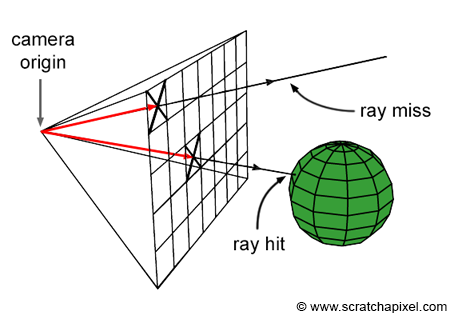
\includegraphics[width=1.0\textwidth]{secciones/imagenes/starting/gpu.png}\label{fig:marcher}
  \caption{Lanzamiento de rayos para el trazado de una escena}
\end{figure}


\section{Spheremarching\label{sec:spheremarching}}
Los algoritmos numéricos suelen ser menos costosos computacionalmente, aproximando con una variable de control que afecta al resultado trazado. En particular, se trata de una técnica reiterativa, conocidas como \textit{Raymarcher}. John C. Hart presentó en 1996 un algoritmo de esta categoría, con el nombre de  \enquote{\textit{Spheremarching}}\cite{hart1996sphere}.\\\\
Esta técnica hace uso las \textit{funciones de distancia con signo} como escena y recibe el atributo de iterativo, ya que, desde la posición de la \textit{cámara} u \textit{ojo}, incrementa el vector director hacia el pixel, conocido como \enquote{rayo} y es proporcional a la \textit{función de distancia con signo} devuelto por el vector iterado. Recibe el prefijo \enquote{\textit{Sphere}\textendash}, ya que, podemos generar, para cada iteracion, una esfera de radio igual al valor de la distancia con signo, sin ningún punto en su interior. Definimos el vector \enquote{rayo} en la iteració n-ésima, como:
\[ \Vec{p}_{n}=\Vec{ojo} + \Vec{direccion} \cdot d_{n} \]
donde \(d_{n}\) es la distancia total recorrida por todas las iteraciones:
\[d_{n}=d_{n-1} + f(\Vec{p}_{n-1})\text{ con } d_0=0\]
Al tratarse de un modelo iterativo, debemos describir las condiciones de parada del algoritmo, donde vamos a destacar tres:
\begin{enumerate}
    \item \textbf{Primera condición}. El algoritmo finalizará cuando estemos \enquote{sobre} la \textit{isosuperficie}. Al tratarse de un algoritmo numérico, vamos a aproximarla, utilizando una variable de control \(\epsilon\) que relajará la restricción de la definición de  \textit{isosuperficie}, haciendo \(f(\Vec{p}_n) < \epsilon\), ya que, si \(\epsilon = 0\), trataríamos de un modelo analítico.
    \item \textbf{Segunda condición}. Superar una cierta distancia recorrida, \(d_{n}\ge MAXIMO\), creando una esfera de trazado sobre el punto de la cámara.
    \item \textbf{Tercera condición}. Superar el número de iteraciones máximas, \(n \ge PASOS\).
\end{enumerate}
Este algoritmo devolverá \(d_n\) para el número de iteraciones fijadas, \enquote{PASOS}. Cuando el algoritmo finaliza debido a la \textbf{segunda o tercera condición}, devolverá, \(d_n=MAXIMO\), recibiendo el nombre de \enquote{\textit{fallo}}. Un fallo, representando un pixel vacío, sin superficie trazada, pudiéndose considerar el fondo de la escena.
 \begin{figure}[H]
  \centering
  \captionsetup{justification=centering}%,margin=2cm
  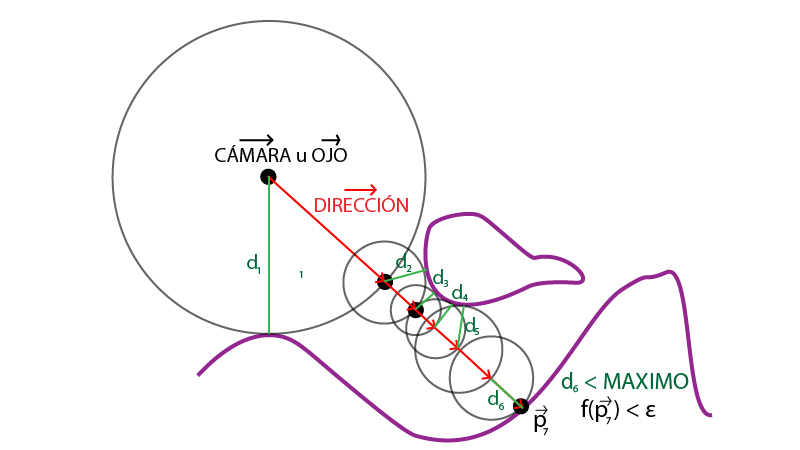
\includegraphics[width=1.0\textwidth]{secciones/imagenes/starting/spheremarching.png}\label{fig:spheremarcher}
  \caption{Ejemplo del algoritmo \textit{Spheremarching}}
\end{figure}

\newpage
\begin{lstlisting}
#define PASOS 128 // Número Máximo de Iteraciones.
#define EPSILON 0.001
#define MAXIMO 20.0 // Distancia del Plano Trasero.

// Pasamos el origen del ojo y la dirección, nos devuelve la distancia al objeto más cercano del ojo en dicha dirección.
float SphereMarching(
    in vec3 ojo, 
    in vec3 direccion
){
    float distancia = 0.0;
    // Realizamos "PASOS" iteraciones de marching.
    for(int i = 0; i < PASOS; ++i){
        // Calculamos el vector (rayo).
        vec3 rayo = ojo + direccion * distancia;
        // Aproximamos el radio de la esfera más próxima a una isosuperficie
        float radio = escena_sdf(rayo);
        // Si el radio (distancia mínima a la isosuperficie), es muy pequeña, podemos decir que estamos sobre la distancia y devolvemos el módulo del rayo.
        if(radio < EPSILON){
            return distancia;
        }
        // Incrementamos la distancia recorrida si no estamos cerca de la isosuperficie.
        distancia += radio;
        // Comprobamos que no se haya superado la distancia de dibujado máximo. Podemos considerarlos el fondo de la escena.
        if(distancia >= MAXIMO) break;
        return MAXIMO;
    }
}
\end{lstlisting}
\newpage
Este algoritmo es implementado en un \textit{shader}, aplicado para cada pixel de nuestra pantalla. En el caso  de que el algoritmo no devuelva \enquote{fallo}, podremos calcular a partir del valor devuelto \(d_n<MAXIMO\) el punto aproximado sobre la superficie, tal que:
\[ \Vec{p} = \Vec{ojo} + d_n \cdot  \Vec{direccion} \]
Conociendo los puntos de una superficie, podremos añadir información a la escena, como por ejemplo, un modelo de iluminación o materiales y texturas.\\\\
En \textit{Shadertoy}, crearemos un nuevo \textit{shader} donde se nos ofrecerá un entorno para trabajar y un código de ejemplo:
\begin{lstlisting}
void mainImage( out vec4 fragColor, in vec2 fragCoord )
{
    // Normalized pixel coordinates (from 0 to 1)
    vec2 uv = fragCoord/iResolution.xy;

    // Time varying pixel color
    vec3 col = 0.5 + 0.5*cos(iTime+uv.xyx+vec3(0,2,4));

    // Output to screen
    fragColor = vec4(col,1.0);
}
\end{lstlisting}
Observamos en el código tres variables enlazadas\ref{sec:enlaces} importante:
\begin{enumerate}
    \item \textbf{out vec4 \textit{fragColor}}. Enlaza la variable con el valor del pixel, una 4-upla, \textit{rgba}, cuyas componentes están en el intervalo \([0,1]\).
    \item \textbf{in vec2 \textit{fragCoord}}. Contiene la posición de la coordenada del pixel en pantalla, donde la primera componente representa la coordenada \(x\) y la segunda, la \(y\).
    \item \textbf{uniform vec2 \textit{iResolution}}. Se trata de una variable global que contiene información de las dimensiones en píxeles del \textit{viewport}, su primera componente, el ancho y su segunda, el alto.
\end{enumerate}
Vamos a modificar el ejemplo anterior: Situraremos la pantalla en la escena, posicionandola centrada en las coordenadas \((0,0,0)\) y preservando la relación de aspecto.  Asignaremos la posición de la cámara u ojo y calcularemos la dirección del ojo al pixel como dirección del rayo. Aplicaremos el algoritmo \textit{spheremarching} desde el ojo en la dirección calculada, en caso de devolver un fallo, utilizaremos el color negro, por el contrario, el blanco.
\newpage
\begin{lstlisting}
void mainImage(
    out vec4 fragColor, 
    in vec2 fragCoord
){
    // Normalizamos las coordendas y las reescalamos para mantener el ratio de aspecto. Transladamos al centro de la pantalla.
    vec2 uv = (fragCoord - iResolution.xy*.5) / min(iResolution.y, iResolution.x);
    // Definimos el ojo y la pantalla, que se encuentra en nuestra escena.
    vec3 ojo = vec3(0.0, 0.0, -1.0);
    vec3 pantalla = vec3(uv, 0.0);
    // La dirección del rayo es el vector normalizado que apunta desde el ojo hasta la pantalla (píxel).
    vec3 direccion = normalize(pantalla-ojo);
    // Con esto, ya podemos utilizar nuestro Sphere marcher.
    float distancia = SphereMarching(ojo, direccion);
    // El marcher nos ha devuelto una distancia inferior al plano trasero, estamos sobre la isosuperficie.
    if(distancia < MAXIMO){
        // Estamos aproximadamente sobre la isosuperficie.
        // La posición aproximada es la siguiente.
        vec3 p = ojo + direccion * distancia;
        // Utilizamos el color blanco para dibujar la isosuperficie.
        fragColor = vec4(1.0);
    }else{ // El marcher ha fallado.
        // El color negro para pintar el fondo.
        fragColor = vec4(vec3(0.0), 1.0);
    }
}
\end{lstlisting}
\newpage
La función \textit{escena\_sdf}, que se encuentra dentro de la función \textit{SphereMarching}, contiene la escena como una \textit{función de distancia con signo}. Veremos en el sexto capítulo\ref{ch:fds}, como crear nuestras escenas. Aunque, para probar nuestro algoritmo, vamos a definir una escena muy simple:
\begin{lstlisting}
/* 
Una esfera en el la coordenada (0,0,0) de radio 0.2 unidades.
*/
float escena_sdf(vec3 p){
    return length(p - vec3(0.0)) - 0.2;
}
\end{lstlisting}
Demos una pincelada de como se ha definido esta función, se calcula el módulo del punto \(\Vec{p}\), esto define una \textit{Función de Distancia} y cuya isosuperficie es únicamente un punto, \(S=\{(0,0,0)\}\), si a cada punto, restáramos \(r\) al la distancia, creamos una isosuperficie esférica de radio \(r\). Ya que, aquellos puntos cuya distancias valen \(r\), acabarán anulándose y definiendo una \textit{función de distancia con signo}.
\[S=\{\Vec{q} \in \mathbb{R}^3 / SDFEsfera_r(\Vec{q})=0\}\]
\[ SDFEsfera_r(\Vec{p})=\vert\vert\Vec{p}\vert\vert - r  \]
\begin{figure}[H]
  \centering
  \captionsetup{justification=centering}%,margin=2cm
  
\includegraphics[width=1.0\textwidth]{secciones/imagenes/starting/sdf1.png}\label{fig:hello}
  \caption{"Hola mundo" del algoritmo \textit{SDF}.}
\end{figure}

Enlace del ejemplo \url{https://www.shadertoy.com/view/wtsfDn}\\\\
Al solo utilizar dos colores, blanco y negro, no tenemos sensación de profundidad, esto se conseguirá definiendo un modelo de iluminación.
    
    % Modelo de iluminacion
    \chapter{Modelo de iluminación}
\section{Introducción}
En este capítulo vamos a ver los principios de los modelos de iluminación, así como operadores importantes. Seguidamente presentaremos el modelo de iluminación Phong, que es y ha sido utilizado desde los años 70.\\\\Un modelo de iluminación es esencial para el diseño artístico de la escena, simular propiedades físicas como por ejemplo, reflejos, refracción, etc. Además, las sombras dan sensación de profundidad a una escena.\\\\
En este capítulo hablaremos de dos elementos importantes, luces y sombras. Aunque no lo parezca, todos ellos hacen uso de una propiedad fundamental de las superficies, el vector normal. Vamos a crear el algoritmo definidio en el apatartado \textit{Preliminares}.
\begin{lstlisting}
// Cálculo de la normal de la isosuperficie estimado por un rayo.
vec3 Normal(vec3 p){
     // f(x1,...,xn)
     float fxyz = escena_sdf(p);
     // f(x1,..,xi+h,xn)
     float fxhyz = escena_sdf(p + vec3(EPSILON, 0.0, 0.0));
     float fxyhz = escena_sdf(p + vec3(0.0, EPSILON, 0.0));
     float fxyzh = escena_sdf(p + vec3(0.0, 0.0, EPSILON));
     // Utilizamos la definicion de derivadas parciales para devolver el gradiente, que se trata de la normal de la isosuperficie, como hemos definido en los Preliminares.
     return vec3(
         (fxhyz - fxyz) / EPSILON,
         (fxyhz - fxyz) / EPSILON,
         (fxyzh - fxyz) / EPSILON
     );
}
\end{lstlisting}
\newpage
Vamos a ahora a presentar el \textit{producto escalar}, implementado de forma nativa en \textit{GLSL} con el nombre de "\textit{dot}", esencial para los modelos de iluminación.
\[\Vec{r} \cdot  \Vec{v} = r_xv_x + r_yv_y + r_zv_z = \vert r\vert\vert v\vert\cos(\alpha)\]
Si ambos son vectores directores, es decir, normalizados y en el origen, resulta \(\Vec{r} \cdot \Vec{v} = \cos(\alpha)\). El valor \(\alpha\) es el ángulo entre los dos vectores sobre el plano que forman, en caso de \(\mathbb{R}^2\), la componente \(z\) sería nula. La imagen del operador es el intervalo \([-1,1]\)\\Veamos alguna de las propiedades, si ambos vectores son perpendiculares, con \(\alpha=\pm\dfrac{\pi}{2}\), el \textit{producto escalar} será \(\Vec{r}\cdot\Vec{v}=\cos\left(\pm\dfrac{\pi}{2}\right)=0\). En el caso en el que sean son paralelos, \(\alpha=\{0,\pi\}\), el resultado será  \(\Vec{r}\cdot\Vec{v}=\cos(\{0, \pi\})=\pm 1\), según la dirección de ambos.\\\\ El lenguaje \textit{GLSL} presenta dos operaciones vectoriales que utilizaremos en modelo, estas son.
%https://es.m.wikipedia.org/wiki/Ley_de_Snell
\begin{table}[h]
    \begin{tabularx}{\textwidth}{l|X}
        \toprule
        Función & Definición\\
        \midrule
        \pbox{10cm}{
          reflect(\\
          \tab[1cm]vecN a,\\
          \tab[1cm]vecN n, \\
          )} & El vector \(\Vec{n}\) debe estar normalizado, este operador devuelve el vector \(\Vec{a}\) reflectado respecto de \(\Vec{n}\),
        \[\Vec{r}=\Vec{a} - 2(\Vec{n} \cdot \Vec{a})\Vec{n}\]
        \begin{minipage}{1.0\textwidth}
          \centering
          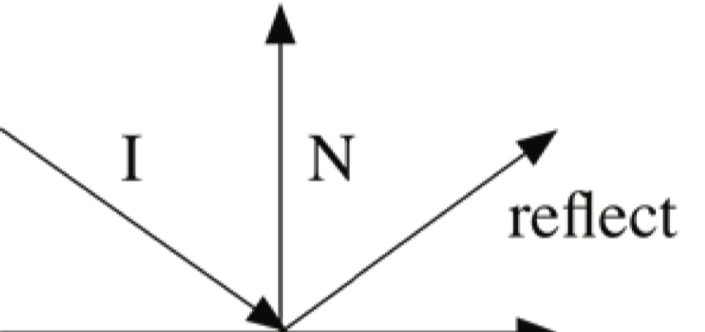
\includegraphics[width=.25\textwidth]{secciones/imagenes/reflect.jpeg}
        \end{minipage}
        \\
        \pbox{10cm}{
        refract(\\
          \tab[1cm]vecN a,\\
          \tab[1cm]vecN n, \\
          \tab[1cm]float k, \\
          )} & El vector \(\Vec{n}\) debe estar normalizado, este operador devuelve el vector \(\Vec{a}\) refractado respecto de \(\Vec{n}\), con \(k\) como factor de medio. Según la \textit{ley de refracción de Snell-Descartes}.
        \[\Vec{r}=k\left(\Vec{a} - \left(\left(\Vec{n} \cdot \Vec{a}\right)+\sqrt{\dfrac{1}{k^2}-(\Vec{a}\cdot\Vec{n})^2}\right)\Vec{n}\right)\]
        \begin{minipage}{1.0\textwidth}
          \centering
          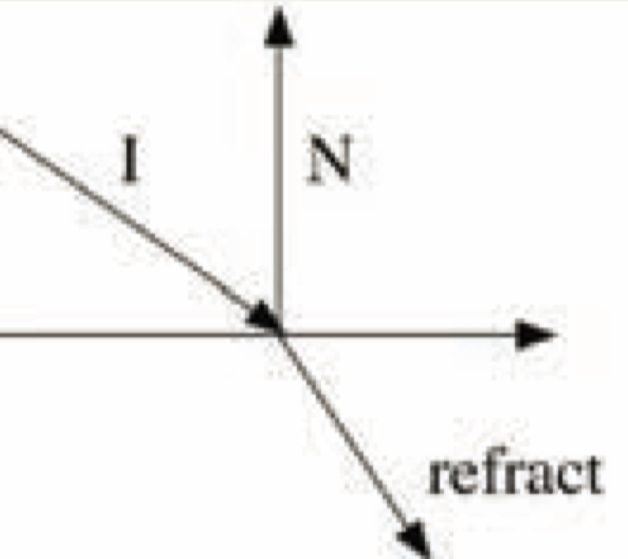
\includegraphics[width=.3\textwidth]{secciones/imagenes/refract.jpeg}
        \end{minipage}\\
        \bottomrule
    \end{tabularx}
\end{table}
\newpage
\section{Luz e Intensidad}
En este apartado veremos la definición de \textit{Intensidad lumínica}, así como dos tipos de luces existentes, luz direccional y radial.\\\\
 Definimos la \textit{intensidad lumínica} en un punto como un factor multiplicativo al material asignado al punto de la \textit{isosuperficie}, representa cómo de iluminado está. Como es un factor multiplicativo, el valor de \(0.0\), representa la intensidad nula u oscuridad. Mientras que el valor \(1.0\) representa el valor más iluminado.\\\\ 
El operador \textit{producto escalar} nos debería dar una breve intuición del papel importante que juega en el cálculo de la intensidad. Como esta no puede ser negativa, definimos el operador producto escalar positivo y normalizado "\(\cdot_{[0,1]}\)".
\[\cdot_{[0,1]}:\mathbb{R}^2\times\mathbb{R}^2\longrightarrow[0,1] : \Vec{a}\cdot_{[0,1]}\Vec{b}=\max\left(\dfrac{\Vec{a}\cdot \Vec{b}}{\vert\vert\Vec{a}\vert\vert\vert\vert \Vec{b}\vert\vert}, 0\right)\]
Vamos a utilizar el "\textit{Modelo de Iluminación de Phong}", presentado en 1973 por \textit{Tuong Phong} como un modelo de iluminación empírico. Para ello, vamos a ver como el modelo se descompone en tres etapas. La primera, el cálculo de la \textbf{Intensidad Ambiente}, que se trata de un valor \(I_a \in [0,1]\) que indica cuanto de iluminada está la isosuperficie, de manera inicial o si no hubieran luces. 
\begin{figure}[H]
  \centering
  \captionsetup{justification=centering}%,margin=2cm
  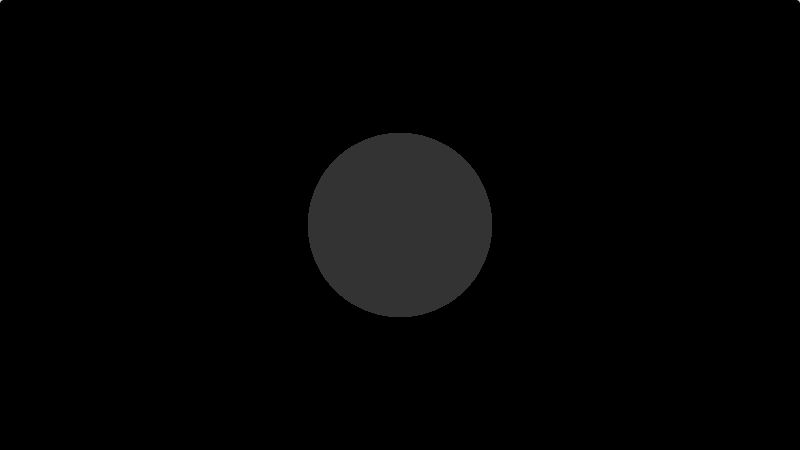
\includegraphics[width=0.8\textwidth]{secciones/imagenes/lightmodel/ambiental.png}\label{fig:ambient}
  \caption{Intensidad Ambiental sobre la esfera.}
\end{figure}
Por otro lado, la \textbf{Intensidad Especular}, que es aportada de manera colectiva sobre el punto aproximado \(\Vec{p}\) de la \textit{isosuperficie}, para cada una de las luces de la escena \(\Vec{l_i}\in L\), donde \(\Vec{l_i}\) representa la posición de la luz, se comprueba como incide la luz sobre la superficie, con respecto de su normal. 
\[I_d = \sum_{\Vec{l_i}\in L} \Vec{n}\cdot_{[0, 1]}(\Vec{l_i}-\Vec{p})\]
Donde \(\Vec{n}\) es la normal de la \textit{isosuperficie} en el punto \(\Vec{p}\). Es fácil observar que, la intensidad debería ser máxima cuando los rayos inciden en de manera paralela en sentido contrario al vector normal y nulo en caso de que sean perpendiculares u opuestos.
\begin{figure}[H]
  \centering
  \captionsetup{justification=centering}%,margin=2cm
  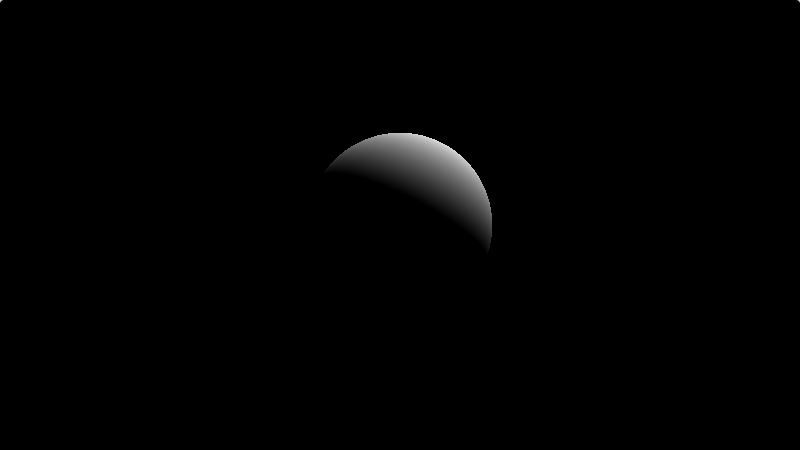
\includegraphics[width=0.8\textwidth]{secciones/imagenes/lightmodel/difusa.png}\label{fig:difusse}
  \caption{Intensidad Difusa sobre la esfera.}
\end{figure}
Veamos finalmente la \textbf{Intensidad Especular}, esta intensidad indica como incide la luz reflectada  por la \textit{isosuperficie} en el la dirección del ojo.\\
Definimos el operador de reflexión "\(\veebar\)"\footnote{La demostración la podemos encontrar en...}, de un vector \(\Vec{a}\) sobre un vector director \(\Vec{n}\).
\[\Vec{a}\veebar\Vec{n}=\Vec{a} - 2(\Vec{n} \cdot \Vec{a})\Vec{n}\]
La ecuación final de la "\textit{Intensidad Especular}" para todas las luces de la escena es,
\[I_e = \sum_{\Vec{l_i}\in L} \Vec{ojo}\cdot_{[0, 1]}\left(\left(\Vec{l_i}-\Vec{p}\right) \veebar \Vec{n}\right)\]
Algunos autores aportan una leve modificación de esta ecuación, aplicando un \textit{homomorfismo} polinómico con grado exponencial.
\[h_k:[0,1]\longrightarrow[0,1] , h_k(x)=x^{2^k}\]
\[I_d = \sum_{\Vec{l_i}\in L} h_k\left(\Vec{ojo}\cdot_{[0, 1]}\left(\left(\Vec{l_i}-\Vec{p}\right) \veebar \Vec{n}\right)\right)\]
Donde \(k\in\mathbb{R}^{+}\) y este tiene efecto sobre el radio de rayos reflejados.
\begin{figure}[H]
  \centering
  \captionsetup{justification=centering}%,margin=2cm
  \subfloat[Intensidad especular con \(h_0\)]{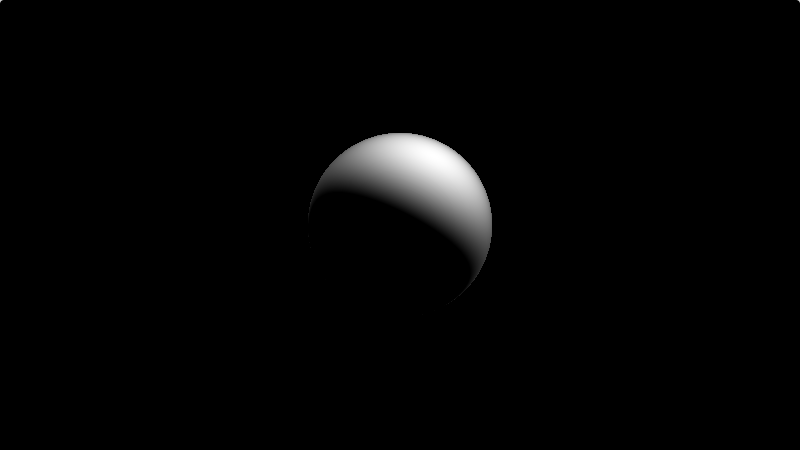
\includegraphics[width=0.33\textwidth]{secciones/imagenes/lightmodel/especular-0.png}\label{fig:specular-0}}
  \subfloat[Intensidad especular con \(h_1\)]{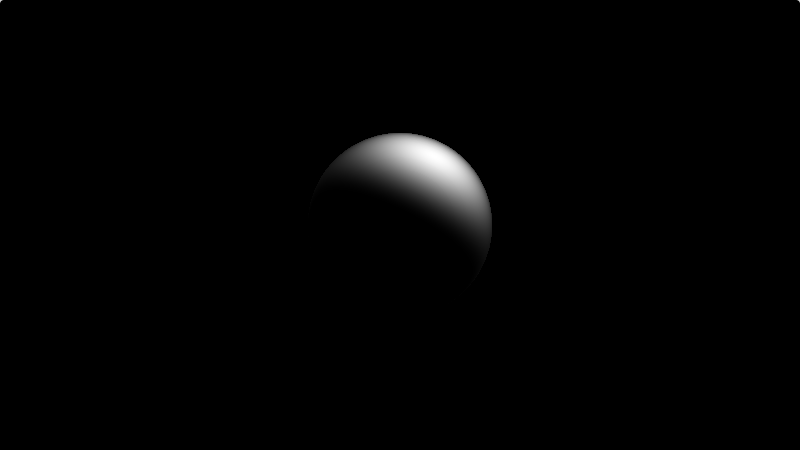
\includegraphics[width=0.33\textwidth]{secciones/imagenes/lightmodel/especular-1.png}\label{fig:specular-1}}
  \subfloat[Intensidad especular con \(h_3\)]{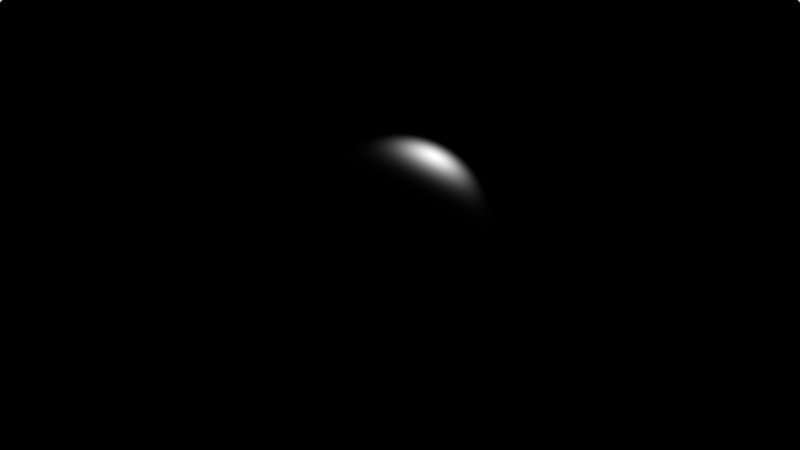
\includegraphics[width=0.33\textwidth]{secciones/imagenes/lightmodel/especular-2.png}\label{fig:specular-2}}
  \caption{Intensidad Difusa con distintos homomorfismos}
\end{figure}
El modelo final, definido por la \textit{Intesidad del modelo de Phong} se calcula como la suma de las intensidades expuestas anteriormente.
\[I_{Phong}=I_a+\sum_{\Vec{l_i}\in L} \mathrlap{\underbrace{\phantom{\Vec{n}\cdot_{[0, 1]}(\Vec{l_i}-\Vec{p})}}_{\text{Intensidad Difusa}}}\Vec{n}\cdot_{[0, 1]}(\Vec{l_i}-\Vec{p}) + \mathrlap{\underbrace{\phantom{h_k\left(\Vec{ojo}\cdot_{[0, 1]}\left(\left(\Vec{l_i}-\Vec{p}\right) \veebar \Vec{n}\right)\right)}}_{\text{Intensidad Especular}}}h_k\left(\Vec{ojo}\cdot_{[0, 1]}\left(\left(\Vec{l_i}-\Vec{p}\right) \veebar \Vec{n}\right)\right)\]
Como hemos dicho antes, este es un factor, multiplicativo, en particular, multiplica al valor del material o en este caso, el color \textit{rgba} devuelto que era, el blanco.
\begin{figure}[H]
  \centering
  \captionsetup{justification=centering}%,margin=2cm
  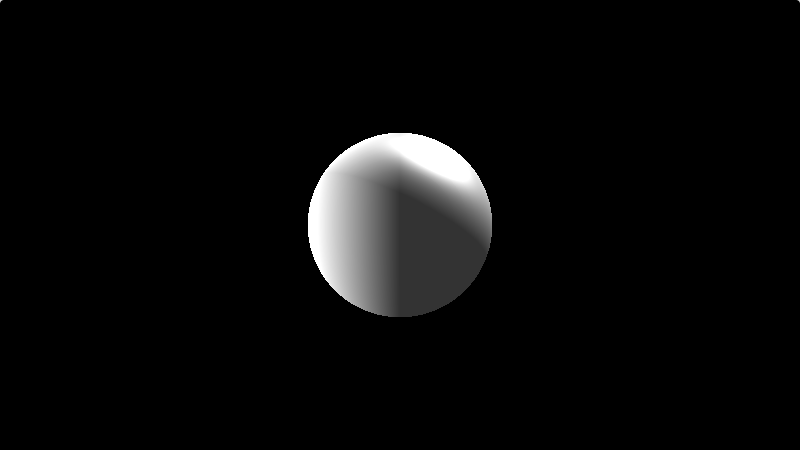
\includegraphics[width=0.8\textwidth]{secciones/imagenes/lightmodel/phong.png}\label{fig:phong}
  \caption{Intensidad Phong sobre la esfera con \(h_3\).}
\end{figure}
En algunas implementaciones, se utiliza para cada luz, un factor de atenuación que depende de la distancia de la superficie a la luz, esta función converge a cero en el infinito. En particular, OpenGL\footnote{A partir de la version X.X empezó...} utiliza la siguiente función:
\[p(x)=\dfrac{1}{ax^2+bx+c}\]
donde \(a,b,c \in \mathbb{R}^{+}_{0}\) son factores que dan una riqueza artística al modelo de iluminación, así como el \textit{homomorfismo} utilizado en la \textit{Intensidad Especular}.\\\\En luces direccionales, el punto se considera estar en el infinito, sustituyéndose \(\Vec{l_i}-\Vec{p}\) por el vector director de la luz \(\Vec{d_i}\). En caso de utilizar una función de atenuación, el valor que tomaría  será cero, por lo que la \textit{Intensidad Especular} quedaría anulada. Además, para la \textit{Intensidad Difusa}, utilizaremos el vector director de la luz direccional en vez de la diferencia del punto aproximado \(\Vec{p}\) y la posición de la luz \(\Vec{l_i}\).
\newpage
Veamos un ejemplo práctico en código.
\begin{lstlisting}
// Homomorfismo
float h3(float h){return pow(h,pow(2.,3.));}
// Definimos el operador producto escalar normalizado positivo.
float dot01(vec3 a, vec3 b){ 
    return max(dot(a,b)/(normalize(a)*normalize(b)), 0.0);
}
// Modelo de iluminación Phong
float ModeloIluminacion(vec3 direccion, vec3 p){
    // Calculamos la normal del punto.
    vec3 normal = Normal(p);
    // Ayuda al marcher a escapar de la isosuperficie
    p = p + normal * 0.1;
    // Modelo
    float intensidad = 0.0;
    // Intensidad Ambiente Global
    intensidad += 0.2;
    // Intensidad de cada Luz
    // Luz 1.
    vec3 posicion_luz_1 = vec3(2., 4., 1.);
    vec3 d_luz_1 = posicion_luz_1 - p;
    float dst_luz_1 = length(d_luz_1);
    // Intensidad Difusa
    intensidad += dot01(d_luz_1, normal);
    // Intensidad Especular, en caso de ser una luz direccional, podemos ignorar esta componente ya que la posición es considerada estar en el infinito y por ello, f_difusa = 0
    vec3 r_luz_1 = reflect(d_luz_1, normal);
    intensidad += f_difusa(dst_luz_1) * h3(dot01(r_luz_1, direccion));
    // ... Utilizamos el mismo esquema para las demás luces.
    // Devolvemos la intensidad en el rango [0, 1].
    return clamp(intensidad, 0.0, 1.0);
}
\end{lstlisting}
\newpage
\section{Sombras}
Vamos a ver la técnica más sencilla para calcular las sombras, pero es importante mencionar que hablaremos únicamente de la \textit{umbra} de una la sombra. La \textit{umbra} sucede cuando la fuente de luz es ocluida completamente por una superficie. Haciendo que la luz no actue sobre la intensidad del punto.\\\\Una vez aproximado un punto \(p\) de la \textit{isosuperficie}, diremos que está en \textit{umbra}, si es ocluido por un objeto en dirección a la luz, o lo que es lo mismo, podemos utilizar el marcher desde \(\Vec{p}\) en dirección a la luz \(\Vec{l_i}\), cuyo plano trasero contiene a \(\Vec{l_i}\). Si este traza otro punto \(\Vec{q}\) en esa dirección, este estará en \textit{umbra}.\\\\
Vamos a realizar una pequeña modificación sobre el vector \(\Vec{p}\) que ayudará a agilizar el \textit{Marcher}, ya que las primeras iteraciones de este, intentará "escapar" de la isosuperficie, para ello, vamos a empujarlo de la superficie, utilizando la normal.
\[\Vec{p'}=\Vec{p} + \Vec{n} \cdot k\]
Donde \(k\in\mathbb{R}^{+}_{0}\) y funciona como un factor de empuje de la superficie, se trata de un valor empírico que ayuda al marcher a salir de la isosuperficie, ya que en las primeras iteraciones, el radio de las esferas está muy próximo a \(0,0\). \\\\
% Imagen Desplazamiento 
Se ha realizado además una leve modificación del marcher, ahora este aceptará un tercer argumento, que indica la distancia del plano trasero, que anteriormente estaba fijado por el plano trasero \textit{MAXIMO}. Esto nos será útil para parar el marcher cuando hemos trazado la distancia la distancia a la luz.\\\\
Vamos a crear un modelo de iluminación con \textbf{dos} luces, una radial y otra direccional. Además, utilizaremos un plano en donde proyectar la sombra. La luz direccional es perpendicular al plano.
\begin{figure}[H]
  \centering
  \captionsetup{justification=centering}%,margin=2cm
  \includegraphics[width=0.8\textwidth]{secciones/imagenes/lightmodel/sombra_dura.png}\label{fig:shadow}
  \caption{Modelo de iluminación y sombras sobre la escena definida.}
\end{figure}
\newpage
\begin{lstlisting}
// Se ha añadido un tercer argumento.
float SphereMarching(in vec3 ojo, in vec3 direccion, float distancia_plano){
    float distancia = 0.0;
    for(int i = 0; i < PASOS; ++i){
        vec3 rayo = ojo + direccion * distancia;
        float radio = escena_sdf(rayo);
        if(radio < EPSILON){
            return distancia;
        }
        distancia += radio;
        // Ahora depende del tercer argumento
        if(distancia > distancia_plano)break;
    }
    return distancia_plano;
}
// Phong + Sombras duras
float ModeloIluminacion(vec3 direccion, vec3 p){
    // Calculamos la normal del punto.
    vec3 normal = Normal(p);
    // Ayuda al marcher a escapar de la isosuperficie
    p = p + normal * 0.1;
    // Modelo
    float intensidad = 0.0;
    // Intensidad Ambiente Global
    intensidad += 0.2;
    // Luz 1.
    vec3 posicion_luz_1 = vec3(2., 4., 1.);
    vec3 d_luz_1 = posicion_luz_1 - p;
    vec3 dir_luz_1 = normalize(d_luz_1);
    float dst_luz_1 = length(d_luz_1);
    // En el caso de que se trate de una luz direccional, utilizaremos el plano MAXIMO, utilizado antes.
    if(SphereMarching(pd, dir_luz_1, dst_luz_1) >= dst_luz_1){
        // Intensidad Difusa
        intensidad += dot01(d_luz_1, normal);
        // Intensidad Especular (Si no es direccional)
        vec3 r_luz_1 = reflect(d_luz_1, normal);
        intensidad += f_difusa(dst_luz_1) * h3(dot01(r_luz_1, direccion));
    }
    // ... Repetimos el esquema anterior.
    return clamp(intensidad, 0.0, 1.0);
}
\end{lstlisting}
%https://www.shadertoy.com/view/wtfBW8
\newpage

    
    % Funciones de distancia con signo
    \section{Funciones de distancia con signo (FDS)}

\SectionPage

\subsection{Primitivas sobre \(\mathbb{R}^2\)}
\begin{frame}[fragile]{Primitivas sobre \(\mathbb{R}^2\)}

    \begin{columns}
        \column{1.5in}
            \begin{figure}[H]
              \centering
              \includegraphics[width=1.0\textwidth]{imagenes/lightmodel/sombra_dura.png}
            \end{figure}
        
        \column{2.5in}
        
            \begin{lstlisting}[boxpos=t]
            float SDFCircunsferencia(vec2 p, float r){
                return length(p) - r;
            }
            \end{lstlisting}
        
    \end{columns}
    
    \begin{columns}
        \column{2.5in}
            \begin{lstlisting}
            float SDFRectangulo(vec2 p, vec2 s){
                vec2 a = abs(p) - s;
                return length(max(a, 0.0)) + min(max(a.x, a.y), 0.0);
            }
            \end{lstlisting}
    
        \column{1.5in}
            \begin{figure}[H]
              \centering
              \includegraphics[width=1.0\textwidth]{imagenes/lightmodel/sombra_dura.png}
            \end{figure}
        
    \end{columns}
    
    \begin{columns}
        \column{1.5in}
            \begin{figure}[H]
              \centering
              \includegraphics[width=1.0\textwidth]{imagenes/lightmodel/sombra_dura.png}
            \end{figure}
        
        \column{2.5in}
            \begin{lstlisting}
            float SDFCircunsferencia(vec2 p, float r){
                return length(p) - r;
            }
            \end{lstlisting}
        
    \end{columns}

\end{frame}

\subsection{Primitivas sobre \(\mathbb{R}^3\)}
\begin{frame}{Primitivas sobre \(\mathbb{R}^3\)}
\end{frame}
    
    % Resolución de Artefactos
    \chapter{Resolución de artefactos}
En el capítulo anterior hemos visto dos tipos de \textit{funciones de distancia con signo} exactas e inexactas. Las funciones exactas devuelven la escena de manera correcta, ignorando imperfecciones por coma flotante. Esto es debido a que la métrica es la euclídea y el \textit{Marcher} siempre traza una esfera con ningún punto en el interior, de ahí su nombre, \textit{Spheremarching}. Cuando tratamos de funciones inexactas, la esferas trazadas también se deforman, por lo que las distancias también lo hacen y por tanto, pueden contener puntos. \\\\
Encontramos dos problemas cuando tratamos de \textit{funciones de distancia con signo inexactas}, en el \textit{Marcher} puede sobreestimar la distancia o subestimar. \\\\

\section{Sobreestimación de la distancia}
Cuando tratamos \textit{funciones de distancia con signo no exactas}, utilizaremos el término \enquote{sobreestimar} cuando se supera la distancia mínima real a la superficie, que es equivalente a que la bola contenga al menos un punto. Encontramos dos formas de  estimar: El rayo trazado se encuentra dentro de la superficie o que el rayo atraviese una superficie. 

\begin{figure}[H]
  \centering
  \subfloat[Se estima dentro de la superficie]{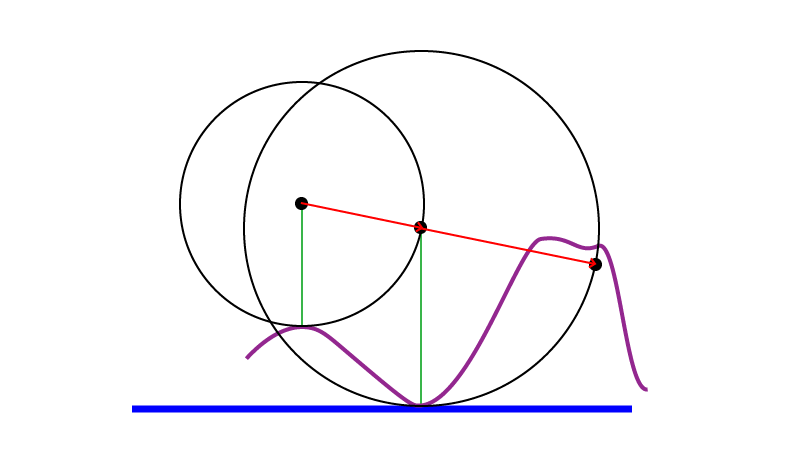
\includegraphics[width=0.45\textwidth]{secciones/imagenes/estimation/sobreestimar-interior.png}\label{fig:estima_dentro}}
  \hfill
  \captionsetup{justification=centering}%,margin=2cm
  \subfloat[Se estima fuera de la superficie]{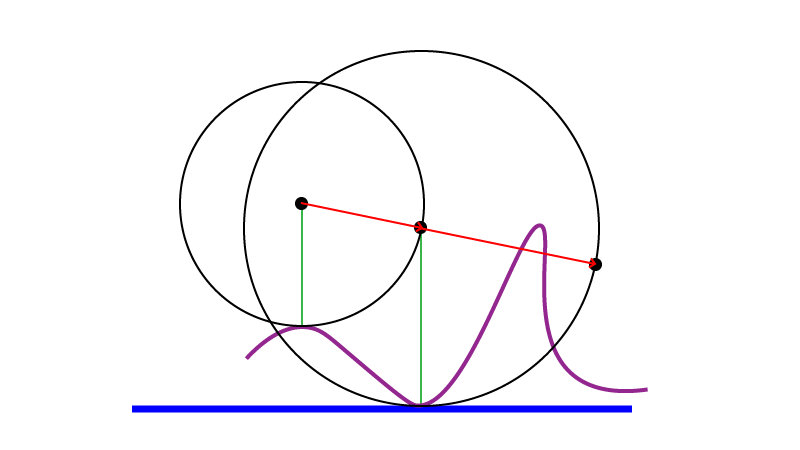
\includegraphics[width=0.45\textwidth]{secciones/imagenes/estimation/sobreestimar-exterior.png}\label{fig:estima_fuera}}
  \caption{Dos formas de sobreestimar una superficie}
\end{figure}

Es difícil visualizar las circunsferencias deformadas, por lo que se ha realizado un esquema de las dos situaciones que podemos encontrar.

\subsection{Sobreestimación dentro de la superficie}
Tenemos definido estar sobre una superficie cuando \(d_{n+1}<\epsilon\), esta restricción había sido elegida ya que \(d_{n+1}\) siempre es positiva cuando trazamos desde fuera de la superficie. Cuando se sobreestima en el interior de la superficie, la siguiente distancia \(d_{n+1}\) será negativa. Debido a la condición de parada anterior, estos puntos del interior son considerados superficie y el algoritmo terminaría. Para solucionarlo, diremos que estamos sobre una superficie, si y solo si, \( \vert d_{n+1} \vert < \epsilon\), este cambio forzará al \textit{Marcher} a que, en caso de estar en el interior de la superficie, el rayo deba salir de la superficie. Veamos el cambio en el código del algoritmo: 
\begin{lstlisting}
float SphereMarching(
    vec3 ojo, 
    vec3 direccion
){
    float distancia = 0.0;
    for(int i = 0; i < PASOS; ++i){
        vec3 p = ojo + direccion * distancia;
        // d_n+1
        float radio = escena_sdf(p);
        // Estamos sobre la superficie cuando aunque sobreestimemos, no estemos <sobre> la superficie. 
        if(abs(radio) < EPSILON){
            return distancia;
        }
        // Cuando d_n+1 sea negativo, intentará escapar del interior hacia el exterior.
        distancia += radio;
        if(distancia >= MAXIMO) break;
    }
    return MAXIMO;
}
\end{lstlisting}

Veamos el efecto que implica este cambio sobre la deformación vista en \fullref{fig:twist}.

\begin{figure}[H]
  \centering
  \captionsetup{justification=centering}%,margin=2cm
  \subfloat[\textit{Marcher} orginal]{
\includegraphics[width=0.45\textwidth]{secciones/imagenes/sdf/3d/sdf_twist.png}\label{fig:twistoriginal}}
  \hfill
  \subfloat[\textit{Marcher} sin sobreestimación en el interior]{
\includegraphics[width=0.45\textwidth]{secciones/imagenes/estimation/sin_sobreestimacion_interior.png}\label{fig:stimateext}}
  \caption{Comparativa de los cambios realizados en el \textit{Marcher}. A la izquierda, el \textit{Marcher} original, a la derecha, el marcher con \(\vert d_{n+1}\vert < \epsilon\)}
\end{figure}

Enlace del ejemplo:\url{https://www.shadertoy.com/view/ttsBDs}

\section{Sobreestimación fuera de la superficie}
Este segundo caso ocurre cuando la deformación aplicada hace que el rayo atraviese la superficie, como ocurre en el ejemplo \textit{(B)}.
Esta sobreestimación afecta considerablemente a la eficiencia del \textit{Marcher}. La solución es escalar en todo momento la bola trazada, obligando a que la bola deformada no pueda contener ningún punto, es decir, sobreestimar. Este cambio nos obligará a utilizar un mayor número de iteraciones, de forma proporcional, para alcanzar la superficie.
\[d'_{n}=d_{n-1} + f(\Vec{p}_{n-1})\cdot k \leq d_{n}\]
Donde \(f\) es nuestra escena; \(k\in[0,1]\) es un factor de escalado de la bola y proporcional al nuevo número de iteraciones. Además, puede ayudar, en ciertas situaciones, a resolver el problema de la \textit{sobreestimación dentro de la superficie}.

\begin{lstlisting}
#define FACTOR_SOBREESTIMACION k
float SphereMarching(
    in vec3 ojo,
    in vec3 direccion, 
    float distancia_plano
){
    float distancia = 0.0;
    for(int i = 0; i < PASOS; ++i){
        vec3 rayo = ojo + direccion * distancia;
        // Escalamos el radio de la esfera
        float radio = escena_sdf(rayo) * FACTOR_SOBREESTIMACION;
        if(abs(radio) < EPSILON){
            return distancia;
        }
        distancia += radio;
        if(distancia > distancia_plano)break;
    }
    return distancia_plano;
}
\end{lstlisting}
Efecto de distintos factores \(k\) al trazado de la escena por el \textit{Marcher}.

\begin{figure}[H]
  \centering
  \captionsetup{justification=centering}%,margin=2cm
  \subfloat[k=1.0]{
\includegraphics[width=0.3\textwidth]{secciones/imagenes/estimation/sin_sobreestimacion_interior.png}\label{fig:twistoriginal1}}
  \hfill
  \subfloat[k=0.75]{
\includegraphics[width=0.3\textwidth]{secciones/imagenes/estimation/sobreestimacion_75.png}\label{fig:twist75}}
  \hfill
  \subfloat[k=0.50]{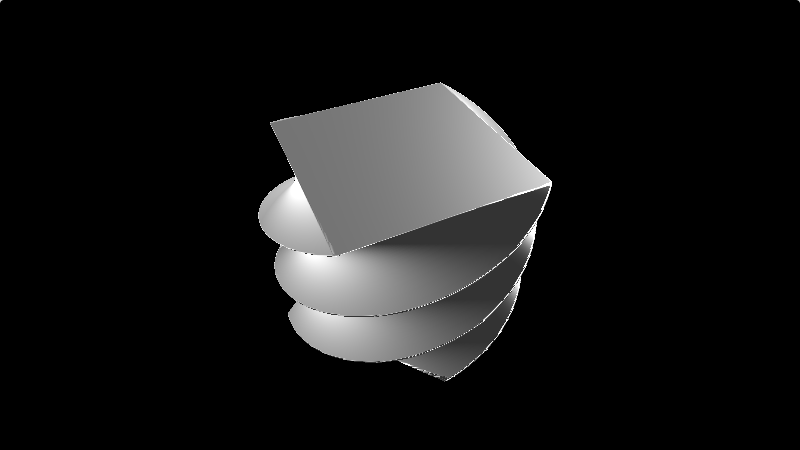
\includegraphics[width=0.3\textwidth]{secciones/imagenes/estimation/sobreestimacion_50.png}\label{fig:twist50}}
  \caption{\(k\in\{1, 0.75, 0.5\}\) respectivamente sobre el \textit{Marcher}}
\end{figure}

Enlace del ejemplo:
\url{https://www.shadertoy.com/view/3tBBRR}

%Vemos que la figura es \enquote{exacta} con \(k=0.5\) si observamos la esquina inferior izquierda de la tapadera. Este factor, o reducción de la esfera a la mitad, va a provocar que se requiera el doble de iteraciones para trazar una escena.

\subsection{Subestimación de la distancia}
Esta estimación puede ocurrir tanto en \textit{funciones de distancia con signo exactas e inexactas}. Ocurre cuando el \textit{Marcher} ha finalizado pero la distancia recorrida por el rayo es inferior a la del plano trasero, es decir, el rayo sigue estando presente en la escena. Por ejemplo, puede ocurrir cuando el rayo pasa de manera paralela, muy cerca a una superficie. Pero, en realidad, no está \enquote{sobre} ella, es decir, \(f(\Vec{rayo}) \ge \epsilon\). La siguiente imagen ilustra este problema:

\begin{figure}[H]
  \centering
  \captionsetup{justification=centering}%,margin=2cm
  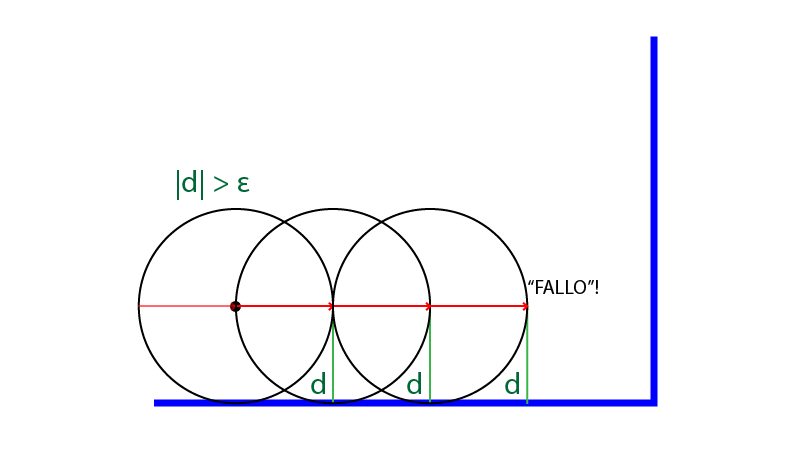
\includegraphics[width=1.0\textwidth]{secciones/imagenes/estimation/subestimacion.png}\label{fig:subestimacion}
  \caption{Ejemplo de subestimación de una superficie}
\end{figure}

Estos puntos serán tratados como \enquote{\textit{fallos}} y por tanto, como píxeles de fondo. Utilizar un factor de sobreestimación \(k > 1\) no sería la solución, ya que, crearía \textit{artefactos}. La principal solución es incrementar el número de iteraciones del algoritmo, es decir, incrementar el número de \enquote{\textit{PASOS}}, provocando un mayor gasto computacional.
    
    % Materiales
    \chapter{Materiales}
En este último capítulo vamos a ver como dar color y texturas a los elementos de nuestra escena. Identificaremos cada elemento asignando un entero positivo \(id \in \mathbb{N}\) que será devuelto junto con la distancia a este objeto, es decir, vamos a devolver un \textit{vec2} cuya componente \enquote{x} será la distancia y cuya componente \enquote{y}, el identificador \(id\). Asignaremos la constante \(id=-1\) cuando no hemos trazado ningún objeto.\\\\
En primer luegar, vamos a modificar el \textit{Marcher} para que este pueda devolver ambos valores:

\begin{lstlisting}
// Devolvemos dos elementos, distancia e id.
vec2 SphereMarching(vec3 ojo, vec3 direccion){
    float distancia = 0.0;
    // Realizamos PASOS iteraciones de marching.
    for(int i = 0; i < PASOS; ++i){
        vec3 p = ojo + direccion * distancia;
        // La escena devuelve el radio de la bola y el id del elemento
        vec2 info = escena_sdf(p);
        // info.x contiene la distancia
        if(info.x < EPSILON){
            // info.y contiene el id de un elemento de la escena.
            // Devolvemos la distancia acumulada (o distancia del ojo a la superficie) y el id.
            return vec2(distancia, info.y);
        }
        // incrementamos la distancia
        distancia += info.x;
        if(distancia >= MAXIMO) break;
    }
    // Devolvemos un id desconocido.
    return vec2(MAXIMO, -1);
}
\end{lstlisting}

El vector devuelto con nombre \textit{info} toma los valores directamente de la escena, por lo que vamos a modificar el esquema de nuestra función \enquote{\textit{escena\_sdf}}, este ahora devolverá la distancia más cercana a un objeto y su identificador. El esquema será el siguiente:

\begin{lstlisting}
vec2 escena_sdf(vec3 p){
    // Identificador inicial y la distancia máxima.
    float id = -1.0;
    float min_dist = MAXIMO;
    
    // El esquema es el siguiente para cada figura de nuestra escena.
    // 1. Creamos nuestra primera figura.
    float sdf_0 = ....;
    // 2. Comprobamos que esta figura es la más cercana encontrada hasta el momento.
    if(sdf_0 < min_dist){
        // 2.1 En caso afirmativo, actualizamos los valores.
        // Asignamos el id de esta figura.
        id = 0.;
        // Actualizamos la distancia mínima como la distancia a esa figura.
        min_dist = sdf_0;
    }
    
    // Repetimos este esquema para cada elemento de la escena,
    float sdf_1 = ...;
    if(sdf_1 < min_dist){
        id = 1.;
        min_dist = sdf_1;
    }
    ...
    // Finalmente, devolvemos la distancia mínima y el objeto que la devuelve.
    return vec2(min_dist, id);
}
\end{lstlisting}

Al devolver ahora dos componentes, debemos modificar todas las funciones que llaman a esta función, encontramos el cálculo de la normal:

\begin{lstlisting}
// En escena_sdf, tomamos la primera componente.
vec3 Normal(vec3 rayo){
     // f(x1,...,xn)
     float fxyz = escena_sdf(rayo).x;
     // f(x1,..,xi+h,xn)
     float fxhyz = escena_sdf(rayo + vec3(EPSILON, 0.0, 0.0)).x;
     float fxyhz = escena_sdf(rayo + vec3(0.0, EPSILON, 0.0)).x;
     float fxyzh = escena_sdf(rayo + vec3(0.0, 0.0, EPSILON)).x;
     
     // Utilizamos la definicion de derivadas parciales para devolver el gradiente, que se trata de la normal de la isosuperficie.
     return vec3(
         (fxhyz - fxyz) / EPSILON,
         (fxyhz - fxyz) / EPSILON,
         (fxyzh - fxyz) / EPSILON
     );
}
\end{lstlisting}

Pongamos como ejemplo una sección de un toro y una esfera, el código y apliquemos el esquema utilizado para \enquote{\textit{escena\_sdf}}. El resultado:

\begin{lstlisting}
vec2 escena_sdf(vec3 p){
    // Identificador inicial y distancia máxima.
    float id = -1.0;
    float min_dist = MAXIMO;
    // Toro de radio interno 0.3 y radio externo 0.05.
    // Seccionado por un plano n = -z.
    // Rotamos el toro 
    vec3 pr = rotYZ(p, PI / 4.);
    float sdf_0 = max(
        SDFToro(pr, 0.3, 0.05),
        SDFPlano(p, vec3(0., 0., -1.))
    );
    // Comprobamos que sea la mas cercana.
    if(sdf_0 < min_dist){
        // Identificador del toro
        id = 0.;
        min_dist = sdf_0;
    }
    // Esfera de radio 0.2
    float sdf_1 = SDFEsfera(p, 0.2);
    // Comprobamos que sea la mas cercana.
    if(sdf_1 < min_dist){
        // identificador de la esfera.
        id = 1.;
        min_dist = sdf_1;
    }
    // Finalmente, devolvemos la distancia mínima y el objeto que la devuelve.
    return vec2(min_dist, id);
}
\end{lstlisting}


\begin{figure}[H]
  \centering
  \captionsetup{justification=centering}%,margin=2cm
  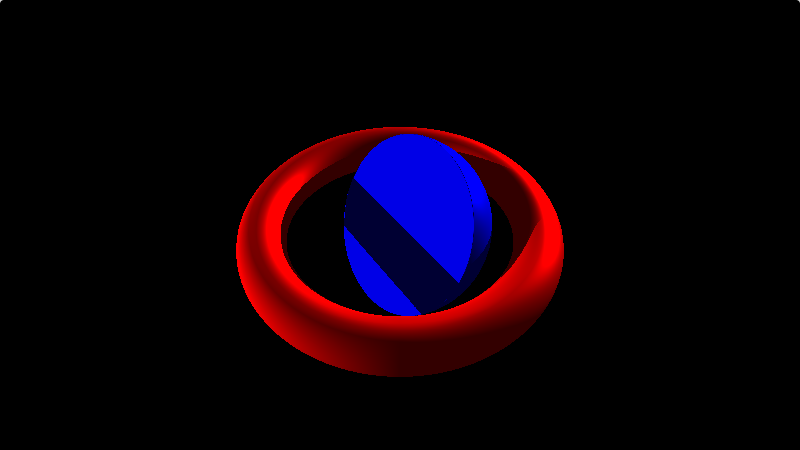
\includegraphics[width=1.0\textwidth]{secciones/imagenes/material/materiales.png}\label{fig:material}
  \caption{Materiales asignados a las distintas figuras.}
\end{figure}

% https://www.shadertoy.com/view/wlBBRR
    
    % Conclusion
    \section{Conclusiones}

\begin{frame}{Conclusiones}
    % \begin{itemize}
    %     \item
    %     Bullet lists are marked with a red box.
    % \end{itemize}

    % \begin{enumerate}
    %     \item
    %     \label{enum:item}
    %     Numbered lists are marked with a white number inside a red box.
    % \end{enumerate}

    % \begin{description}
    %     \item[Description] highlights important words with red text.
    % \end{description}

    % Items in numbered lists like \enumref{enum:item} can be referenced with a red box.

    % \begin{example}
    %     \begin{itemize}
    %         \item
    %         Lists change colour after the environment.
    %     \end{itemize}
    % \end{example}
\end{frame}

    \begin{frame}[allowframebreaks]{References}
        
        \bibliography{bibliografia.bib}
    	\bibliographystyle{apalike}
    	\printbibliography
        
        La plantilla utilizada:
        \url{https://github.com/martinhelso/UiB}
        
    \end{frame}

\end{document}